El treball presentat en aquesta tesi s'ha desenvolupat en el marc de l'experiment ATLAS del Gran Colisionador de Hadrones (LHC) del CERN, durant els meus estudis de doctorart en l'Institut de Física Corpuscular (IFIC, CSIC–Universitat).
La investigació s'ha centrat en dos objectius complementaris. El primer és el desenvolupament de tècniques avançades d'identificació d'electrons, un ingredient fonamental per a nombroses anàlisis de precicisió i recerques de física nova. 
El segon és l'estudi de processos rars de producció del bosó de Higgs directament sensible a l'acoplament de Yukawa amb el quark top, amb l'especial ènfasi en estats finals amb leptons $\tau$ que es desintegren hadrònicament.

\section*{Introducció al Model Estàndar i Física del bosó de Higgs}

El Model Estàndard de la física de partícula~\cite{Glashow,Weinberg,Salam} constitueix el marc teòric que descriu les partícules elementals conegudes i les seues interaccions fonamentals. exceptuant la gravetat. 
Formulat al llarg de la segona mitat del segle XIX, combina de forma coherent la mecànica quàntica, la relativitat especial i la teoria quàntica de camps. 
Es basa en un grup de simetria gauge \(\mathrm{SU(3)_{C} \times SU(2)_{L} \times U(1)_{Y}}\), el qual correspon a les interaccions fort, feble i electromagnètica, respectivament.

En aquest esquema, els constituyents bàsics de la matèria són els fermions: sis quarks (up, down, charm, strange, top y bottom) i sis leptons (electrón, $\mu$, $\tau$ i els seus neutrins asociats). Aquestos s'organitzen en tres generacions amb propietats anàlogues però masses creixents. La primera generació (u, d, e, \(\nu_{e}\)) conforma la matèria ordinària, mentres que les següents apareixen únicament en condicions d'alta energia, com les alcançades en acceleradors de partícules. 

Les interaccions són mediades per bosons gauge: els gluons en el cas de la interacció fort, els bosons \(W^\pm\) i \(Z\) per a la interacció feble, i el fotó per a la interacció electromagnètica. A més, el Model Estàndar inclou un camp escalar fonamental, el camp de Higgs, 

Un dels aspectes més destacables del Model Estàndard és la seua capacitat per a unificar les interaccions electromagnètica i dèbil en un marc gauge comú, conegut com a teoria electrodèbil~\cite{Glashow,Weinberg,Salam}. No obstant això, les simetries gauge imposen que les partícules associades a aquests camps han de ser sense massa, en contradicció amb l’observació experimental dels bosons vectorials pesats \(W^\pm\) i \(Z\). La solució s’introdueix mitjançant el mecanisme de Higgs~\cite{Brout,HiggsSpontan}: un camp escalar complex amb simetria de gauge \(\mathrm{SU(2)_{L} \times U(1)_{Y}}\), el potencial del qual adopta una forma no trivial, anomenada del "barret mexicà", com es mostra en la Figura~\ref{res:mexican_hat}. Aquesta forma indueix la trencament espontani de la simetria.

\begin{figure}[htbp]
  \centering
  \includegraphics[angle=-90,width=0.7\textwidth]{images/mexican_hat.pdf}
  \caption{Il·lustració de la forma del potencial escalar complex del Higgs, amb $v$ el valor esperat del buit. La simetria es trenca espontàniament quan s’escull un estat fonamental (A $\rightarrow$ B).}
  \label{res:mexican_hat}
\end{figure}

En aquest procés, el camp de Higgs adquireix un valor esperat en el buit distint de zero (VEV, \(\langle H \rangle \approx 246\) GeV). Tres dels quatre graus de llibertat del doblet de Higgs es converteixen en les components longitudinals dels bosons \(W^\pm\) i \(Z\), atorgant-los massa. El grau de llibertat restant correspon al bosó de Higgs físic, la massa del qual va ser mesurada al voltant de \(125\) GeV.  

A més d’explicar l’origen de la massa dels bosons gauge, el mecanisme de Higgs també proporciona un marc per a generar les masses dels fermions. Aquest procés s’implementa mitjançant els acoblaments de Yukawa, que connecten el camp de Higgs amb els fermions de manera proporcional a la seua massa. La força d’aquests acoblaments varia des de valors molt petits per a electrons i neutrins fins a valors de l’ordre de la unitat per al quark top, el fermió més pesat conegut.  

L’acoblament de Yukawa del quark top, \(y_{t}\), és d’un interés particular. La seua magnitud determina directament la probabilitat de processos de producció com el \(\ttH\), en què un Higgs es produeix en associació amb un parell top-antitop, constituint una mesura directa de \(|y_{t}|\). Igualment, la producció associada amb un sol quark top (\(tH\)) presenta una dependència lineal amb l’acoblament de Yukawa del top, a diferència de \ttH, la secció eficaç del qual escala de manera quadràtica. Aquesta característica converteix el procés en un observatori privilegiat per a explorar possibles fases intermèdies de CP en la interacció, ja que la mesura conjunta de \ttH\ i \(tH\) aporta informació complementària sobre l’estructura de l’acoblament del Higgs al top~\cite{Bernreuther:2002uj,Brod:2013cka}.  

Les mesures experimentals de seccions eficaces de producció del bosó de Higgs es poden interpretar dins del marc de les \textit{Simplified Template Cross Sections} (STXS)~\cite{badger2016leshouches2015physics,STXS11}. Aquesta estratègia consisteix a dividir l’espai de fase en regions cinemàtiques ben definides, optimitzades per a maximitzar la sensibilitat experimental i minimitzar les dependències teòriques.  

L’esquema STXS permet combinar de manera coherent resultats de diferents modes de desintegració i de producció, i s’ha convertit en l’estàndard de la Col·laboració ATLAS per a caracteritzar la física del Higgs. En el cas de processos associats al quark top, com \(\ttH\) i \(tH\), les categories STXS diferenciades en bins de moment transversal del Higgs \(p_{\text{T}}^{H}\) són especialment rellevants per a estudiar els acoblaments de Yukawa i millorar la sensibilitat en escenaris de nova física.

\begin{figure}[htbp]
  \centering
  \subfloat[]{
      \includegraphics[width=0.46\textwidth]{atlas_combined_xsect.pdf}
  }
  \hfill
  \subfloat[]{
      \includegraphics[width=0.46\textwidth]{atlas_combined_br.pdf}
  }
  \caption{(a) Resum de les seccions eficaces de producció del bosó de Higgs assumint els valors del Model Estàndard per als \textit{branching ratios} de desintegració.  
  (b) Mesures dels \textit{branching ratios} de desintegració del bosó de Higgs assumint les prediccions del Model Estàndard per a les seccions eficaces de producció.  
  Tots els resultats s’obtenen utilitzant les dades del Run~2 d’ATLAS, combinant diferents anàlisis, i són compatibles amb les prediccions del Model Estàndard dins de les incerteses~\cite{Nature_ATLAS}.}  
  \label{res:higgs_mu}
\end{figure}

L’estudi detallat del bosó de Higgs constitueix una de les principals prioritats del programa de física del LHC. La caracterització dels seus acoblaments amb fermions i bosons vectorials no sols serveix com a prova interna del Model Estàndard, sinó que també obri la porta a explorar possibles desviacions associades a teories més enllà d’aquest, com la supersimetria o els models de Higgs compostos.  

En aquest context, les anàlisis que exploten desintegracions a leptons $\tau$ i la producció associada amb quarks top adquireixen un paper central, en combinar sensibilitat als acoblaments fermiónics de tercera generació amb entorns experimentals complexos.

%%%%%%%%%%%%%%%%%%%%%%%%%%%%%%%%%%%%%%%%%%%%%%%%%%%%%%%%%%%%%%%%%%%%%%%%%%%%%%%%%%%%%%%%%%%%%%%%%%%%%%%%%

\section*{El LHC i el detector ATLAS}

El Gran Col·lisionador d’Hadrons (LHC, per les seues sigles en anglés)~\cite{Evans:1129806, Bruning:782076} és l’accelerador de partícules més potent construït fins ara. Està situat en un túnel circular de 27~km de circumferència, a uns 100~metres de profunditat, a la frontera franco-suïssa, reutilitzant la infraestructura prèvia del \textit{Large Electron–Positron Collider} (LEP). Va ser dissenyat per a col·lisionar protons i ions pesants a energies sense precedents, amb l’objectiu d’explorar el sector del bosó de Higgs, la física de precisió del Model Estàndard i la possible existència de nova física.

Els feixos de protons són injectats en el LHC a través d’un complex de preacceleradors que inclou el \textit{Linac}, el \textit{Proton Synchrotron} (PS) i el \textit{Super Proton Synchrotron} (SPS). Una vegada en l’anell principal, els feixos es mantenen mitjançant 1232 dípols superconductors de 8.3~T que guien la seua trajectòria, i prop de 400 quadrupols que enfoquen el feix. El sistema opera a temperatures criogèniques de 1.9~K utilitzant heli superfluïd.

Durant el Run~2 (2015–2018), el LHC va aconseguir col·lisions protó-protó a $\sqrt{s} = 13$~TeV, amb lluminositats integrades d’aproximadament $140~\text{fb}^{-1}$ per a ATLAS i CMS. En el Run~3 (2022–2025), l’energia de col·lisió ha augmentat fins a 13.6~TeV, amb l’objectiu d’acumular més de $300~\text{fb}^{-1}$. El futur projecte HL-LHC preveu incrementar aquest valor en un factor deu, assolint $3000~\text{fb}^{-1}$ de dades registrades per cada experiment, la qual cosa permetrà explorar processos rars amb una sensibilitat sense precedents.

ATLAS~\cite{ATLAS:exp,ATLAS_run3} és un dels dos detectors generals de propòsit múltiple del LHC. Amb 44~m de longitud, 25~m d’altura i un pes total de 7000~tones, és el detector de major volum construït en un accelerador. El seu disseny en capes concèntriques permet una cobertura quasi completa en angle sòlid, sent capaç de registrar leptons, fotons, jets hadrònics i energia transversal perduda en un ampli rang d’energies.

\begin{center}
  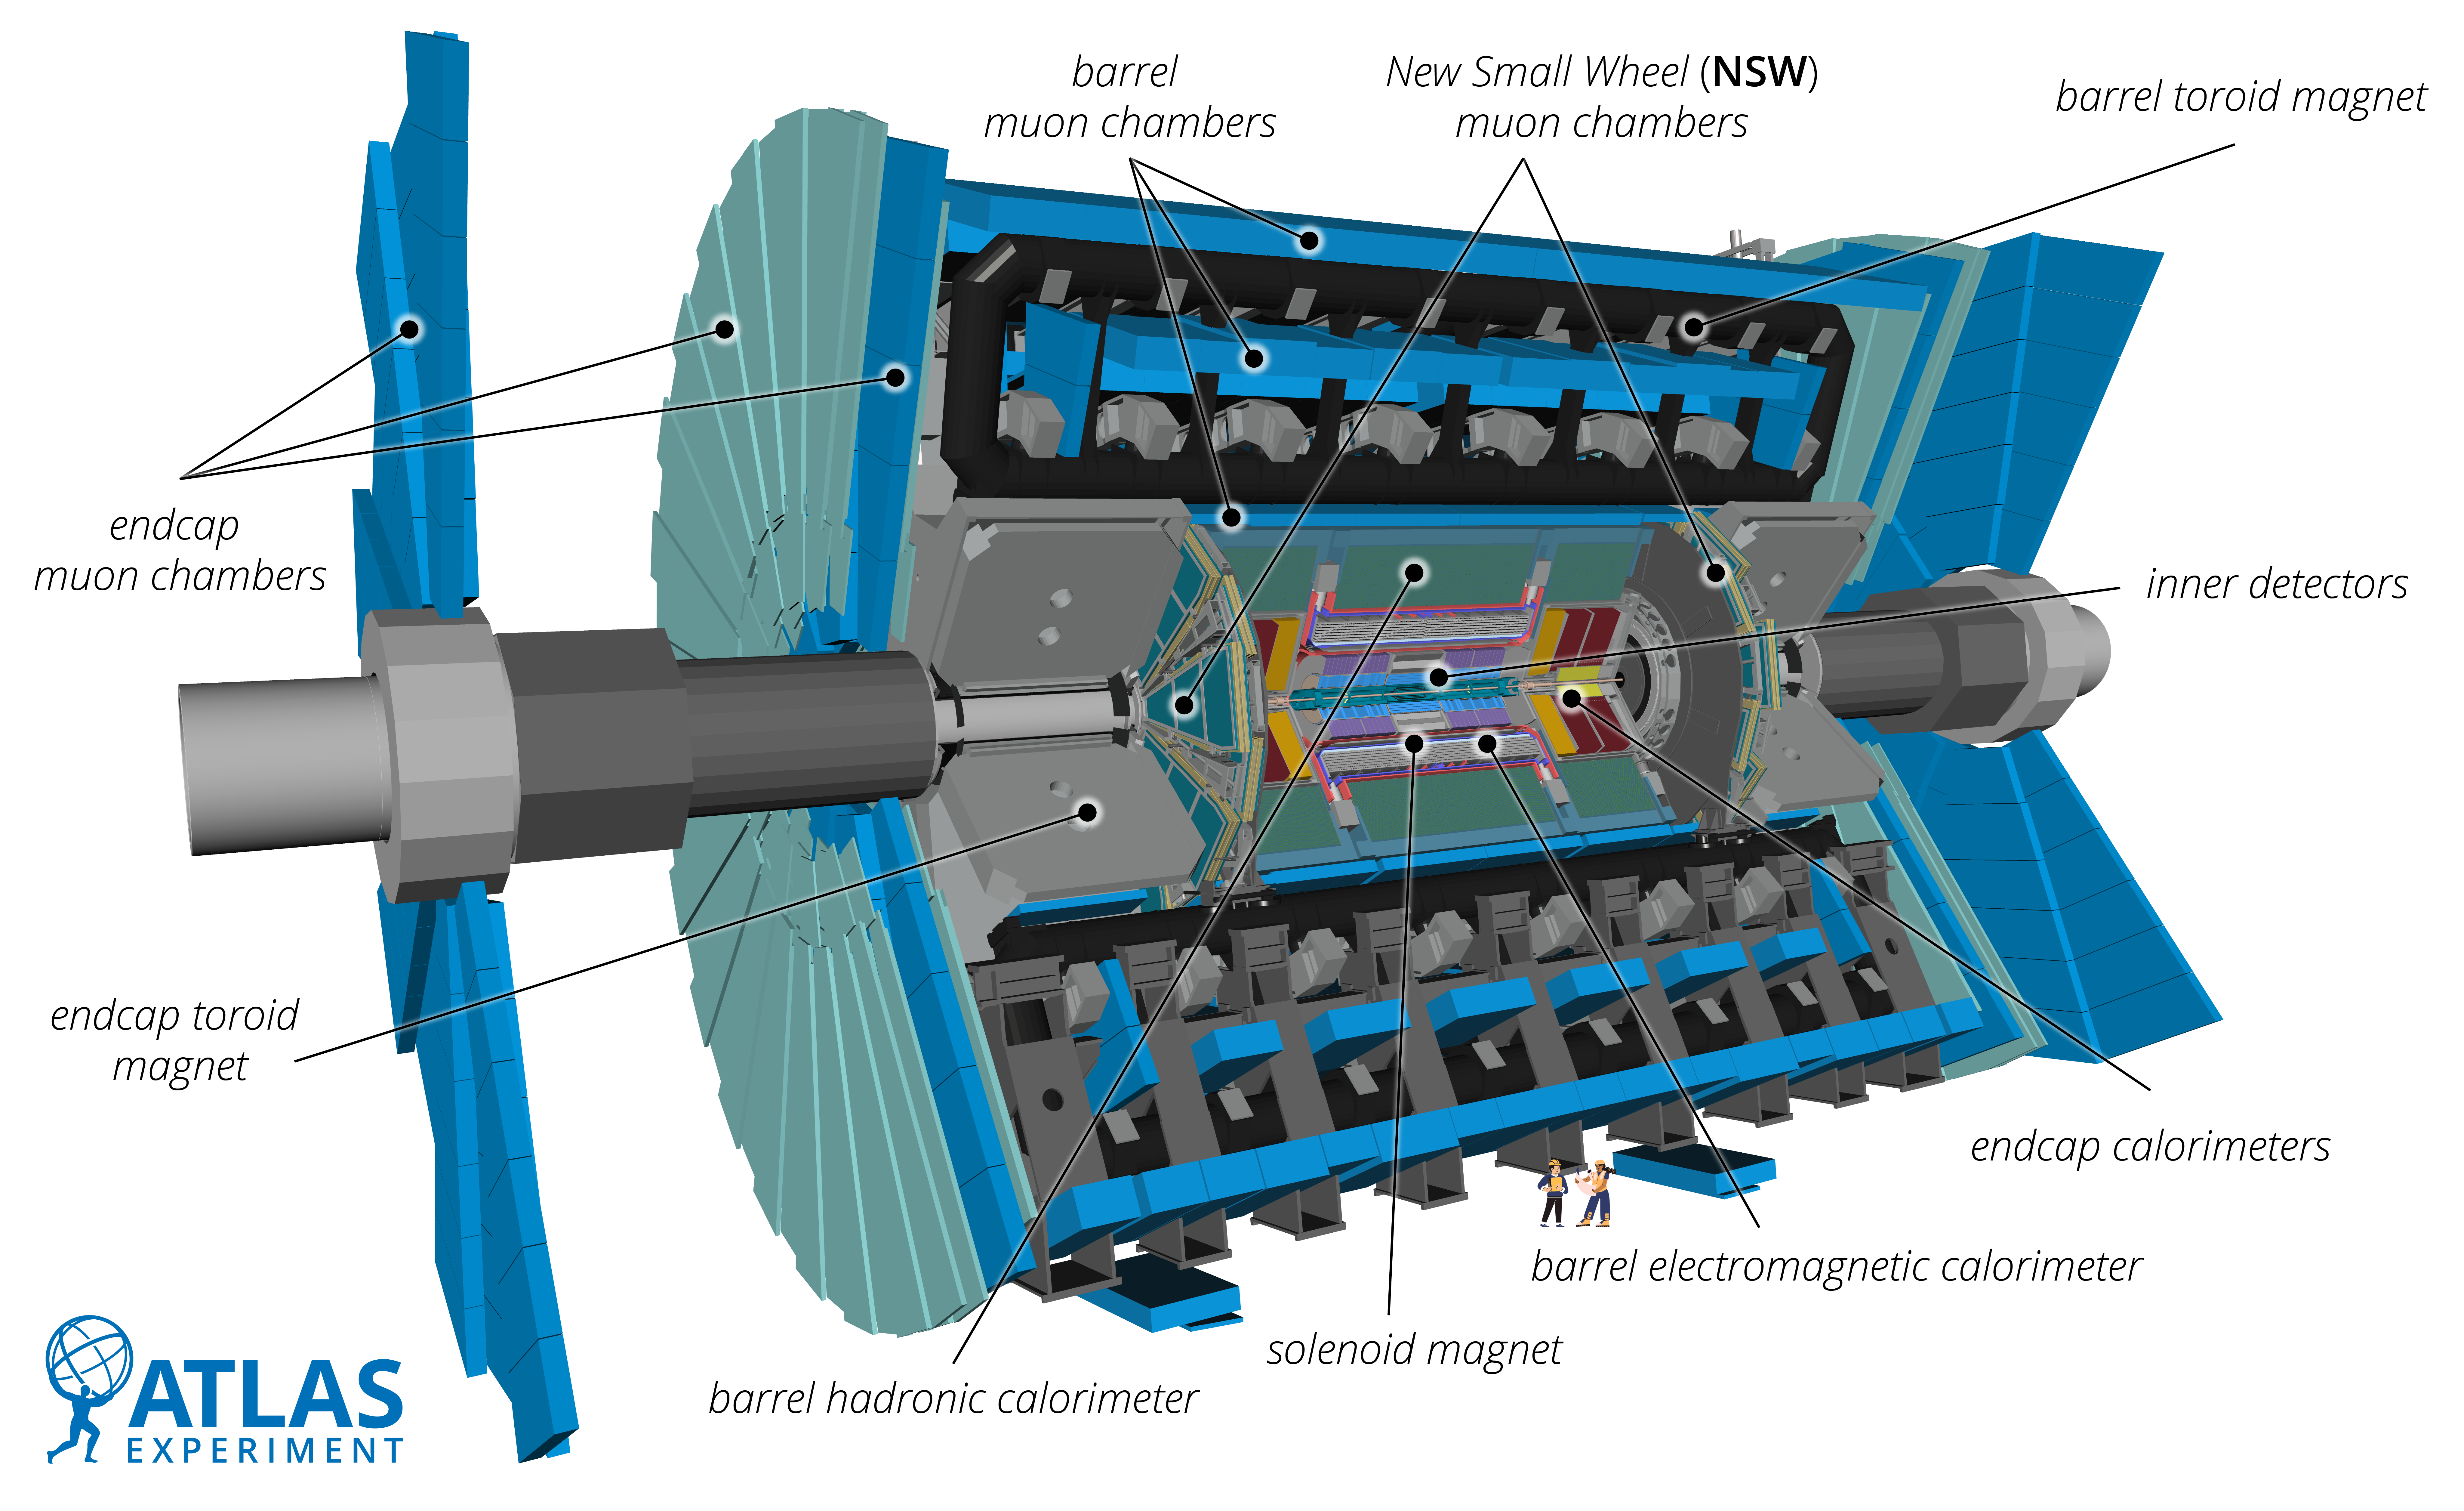
\includegraphics[width=0.75\textwidth]{images/ATLAS-Experiment-Schematic-2022-Labels-People.png}
  \captionof{figure}{Vista esquemàtica del detector ATLAS, que mostra els seus principals subsistemes: detector intern, calorímetres i espectròmetre de muons~\cite{Bianchi:2837191}.}
\end{center}

\textbf{Detector intern (ID)~\cite{2010_id,ATLAS:exp}:} reconstrueix les trajectòries de les partícules carregades en el camp magnètic de 2~T generat per un solenoide superconductor. Inclou el detector de píxels, el SCT de tires de silici i el TRT. És essencial per a les mesures d’impacte, la reconstrucció de vèrtexs i la separació entre electrons i hadrons.  

\textbf{Calorímetres~\cite{2010_lar,2010_tile}:} el calorímetre electromagnètic, basat en argó líquid i plom, ofereix una gran resolució en energia per a electrons i fotons. Els calorímetres hadrònics, formats per rajoles centellejadores i argó líquid amb coure/tungstè, permeten la mesura de jets i d’energia transversal perduda.  

\textbf{Espectròmetre de muons~\cite{muon_com}:} situat a l’exterior del detector i immers en un camp magnètic toroidal de 4~T, detecta els muons que travessen els sistemes de calorimetria. Està compost per quatre subsistemes:  
\textit{Monitored Drift Tubes} (MDT) i \textit{Cathode Strip Chambers} (CSC) per a mesurar el moment, i \textit{Resistive Plate Chambers} (RPC) i \textit{Thin Gap Chambers} (TGC) per a generar senyals de \textit{trigger}.  
La combinació d’aquests subsistemes permet mesurar la curvatura de les trajectòries dels muons.  

\textbf{Detectors \textit{Forward}:} ATLAS disposa de diversos detectors orientats cap a la direcció dels feixos (LUCID~\cite{Jenni:721908}, ALFA~\cite{Khalek_2016}, AFP~\cite{Adamczyk:2015cjy} i ZDC~\cite{Jenni:1009649}) que estenen la cobertura a regions de pseudorapidesa molt alta.  
Aquests sistemes permeten mesurar la lluminositat relativa i absoluta, estudiar processos de dispersió elàstica, detectar protons molt avançats i registrar partícules neutres en col·lisions d’ions pesants.  

\textbf{Trigger~\cite{trigger_run2}:} el sistema de selecció d’esdeveniments en temps real, amb un primer nivell de maquinari (L1) i un nivell posterior basat en software (HLT), redueix la taxa d’esdeveniments de 40~MHz a aproximadament 1~kHz, que s’emmagatzemen per a la seua anàlisi.  

L’anàlisi de les dades registrades per ATLAS requereix una infraestructura computacional de gran escala.  
L’experiment utilitza un sistema de computació distribuïda basat en la \textit{Worldwide LHC Computing Grid} (WLCG)~\cite{Bird:1695401}, que connecta més de 170 centres en 40 països, proporcionant centenars de petabytes de capacitat d’emmagatzematge i una potència de càlcul equivalent a diversos milions de nuclis de CPU.  

El flux de dades segueix un esquema jeràrquic en tres nivells: els \textit{Tier-0} al CERN processen en temps real la reconstrucció inicial; els \textit{Tier-1}, distribuïts internacionalment, emmagatzemen i recalibren les dades; i els \textit{Tier-2} i \textit{Tier-3} ofereixen recursos per a simulacions Monte Carlo (MC) i per a l’anàlisi per part dels físics.  

El software d’ATLAS està basat en el \textit{framework} \textsc{athena}~\cite{athena}, desenvolupat en C++ i Python, que integra la simulació d’esdeveniments, la reconstrucció d’objectes físics i l’aplicació d’algorismes d’identificació.  
Les diferents versions de \textsc{athena}, conegudes com a \textit{releases}, defineixen la configuració oficial de reconstrucció i calibratge utilitzada en cada període de presa de dades.  
En paral·lel, les campanyes de producció MC (MC16 per al Run~2, MC20 i MC23 per al Run~3) proporcionen mostres coherents amb les condicions de detector i de feix en cada època d’operació del LHC.

\section*{Dades i simulacions}

Les anàlisis presentades en aquesta tesi es basen en dades de col·lisions protó-protó registrades per ATLAS en el Run~2 (2015–2018) i el Run~3 (2022–2024), que sumen $140~\text{fb}^{-1}$ a $\sqrt{s}=13$~TeV i uns $166~\text{fb}^{-1}$ a $\sqrt{s}=13.6$~TeV, respectivament, després d’aplicar els criteris de qualitat de dades.  
Aquests conjunts s’utilitzen tant per a validar noves estratègies d’identificació d’electrons com per a estudiar modes poc freqüents de producció del bosó de Higgs, incloent-hi \(\ttH\) i \(tHqb\).  

La modelització de les col·lisions protó-protó en el LHC constitueix un repte essencial, ja que involucra múltiples escales energètiques i processos simultanis~\cite{BUCKLEY2011145}.  
En la QCD perturbativa, els protons es tracten com a feixos de partons (quarks i gluons) descrits per funcions de distribució de partons (PDFs), que defineixen la probabilitat que un partó transporte una fracció $x$ del moment del protó.  
Els càlculs a ordres NLO i NNLO proporcionen les seccions eficaces dels processos durs, combinats amb algorismes de \textit{parton showering} que simulen la cascada de radiació partònica, seguits de la hadronització en estats lligats de color neutre mitjançant models fenomenològics.  
A més, s’inclouen fenòmens col·lectius com les col·lisions múltiples de partons (MPI) i el \textit{pile-up}, és a dir, interaccions simultànies en un mateix encreuament de feixos que afecten la reconstrucció d’objectes físics.  

La simulació d’aquests processos es du a terme mitjançant campanyes de producció Monte Carlo (MC) específiques per a cada època de dades.  
El flux típic consisteix en la generació d’esdeveniments a nivell partònic amb programes com \textsc{powheg}~\cite{Frixione_2007}, \textsc{madgraph5\_amc@nlo}~\cite{Alwall_2014} o \textsc{sherpa}~\cite{Bothmann_2019}, interfaçats amb hadronitzadors com \textsc{pythia8}~\cite{SJOSTRAND2015159} o \textsc{herwig}~\cite{B_hr_2008}, i posteriorment amb la simulació detallada del detector mitjançant \textsc{geant4}~\cite{AGOSTINELLI2003250}.  

En els estudis d’electrons s’utilitzen mostres dedicades de $Z\to e^+e^-$ i $J/\psi \to e^+e^-$, fonamentals per a validar la reconstrucció, estudiar l’eficiència d’identificació i derivar factors d’escala en comparar dades i MC.  
Els principals fons que imiten electrons es modelitzen amb processos multijet QCD, desintegracions d’hadrons pesants ($b$, $c$) i fotons convertits, utilitzant mostres específiques com JF17 generades amb \textsc{pythia}~\cite{SJOSTRAND2015159}.  

En el cas del Higgs, els processos de senyal \(\ttH\) i \(tHqb\) es simulen a precisió NLO o NNLO, incloent-hi la desintegració $H\to\tau\tau$.  
Els fons dominants (\(\ttbar\)+jets, $Z\to\tau\tau$+jets i multijets QCD) es normalitzen a càlculs d’ordre superior quan estan disponibles (NNLO en el cas de Drell–Yan) i a mesures de lluminositat integrada.  
En tots els casos, els esdeveniments MC es corregeixen per a reproduir les condicions reals del detector, incloent-hi calibracions d’energia i resolucions dels diferents objectes físics.

\section*{Reconstrucció d’objectes físics}

Una vegada que el HLT accepta un esdeveniment, les dades registrades en les col·lisions es processen de manera \textit{offline} amb la finalitat de reconstruir les partícules emergents de la interacció protó–protó.  
Els senyals registrats en l’ID, els calorímetres i el MS es combinen mitjançant algorismes dedicats que permeten construir els diferents objectes físics, els quals constitueixen els ingredients essencials de totes les anàlisis realitzades en ATLAS.  
Entre ells s’inclouen les traces carregades i els vèrtexs de col·lisió, muons, electrons i fotons, jets (amb algorismes dedicats per a classificar-los segons el seu sabor), leptons $\tau$ que decauen hadrònicament, així com el moment transversal perdut ($E_{\mathrm{T}}^{\text{miss}}$).  

\begin{figure}[h]
  \centering
  \includegraphics[width=0.9\textwidth]{images/atlas_particles.png}
  \caption{Esquema en el pla $x-y$ de partícules elementals que interaccionen amb els diferents subsistemes del detector ATLAS~\cite{Bianchi:2837191}.}
  \label{res:reco}
 \end{figure}

El primer pas en la reconstrucció és identificar les trajectòries de les partícules carregades que travessen el detector intern~\cite{tracks}.  
Aquestes produeixen impactes precisos en els subdetectors de silici (Pixel, SCT) i en el TRT, que sota el camp magnètic solenoïdal de 2~T es corben descrivint idealment hèlixs.  
Cada traça reconstruïda queda definida per cinc paràmetres: el moment transversal ($p_{\mathrm{T}}$), els angles polars ($\theta, \phi$) i els paràmetres d’impacte transversal i longitudinal ($d_{0}, z_{0}$).  

A partir de les traces, es reconstrueixen els vèrtexs d’interacció~\cite{vertex_run1,vertex_run2,vertex_run3,vertex_run3_2}.  
El vèrtex primari correspon al punt de la col·lisió dura, identificat com aquell amb la major suma de $p_{\mathrm{T}}^{2}$ de les traces associades, mentre que altres vèrtexs es classifiquen com a \textit{pile-up} o secundaris.  
Aquests últims són essencials per a l’etiquetatge de sabor i la identificació de partícules desplaçades.

Després de travessar el detector intern, les partícules dipositen la seua energia en les cel·les dels calorímetres, que s’agrupen en clústers tridimensionals anomenats \textit{topoclusters}.  
L’algorisme comença a partir de cel·les llavor amb senyal significativa respecte al soroll electrònic i s’expandeix iterativament a cel·les adjacents.  
Posteriorment, s’apliquen calibracions específiques que corregeixen les pèrdues en materials passius i la diferent resposta hadrònica i electromagnètica.  
Durant el Run~2 es va introduir a més el concepte de \textit{superclúster}, que agrupa dinàmicament diversos topoclusters, millorant la recuperació d’energia perduda per radiació de bremsstrahlung.

Els muons es reconstrueixen combinant informació de l’ID i del MS~\cite{muon_reco_run2}, atés el seu caràcter de partícules mínimament ionitzants que travessen el detector amb una pèrdua d’energia reduïda.  
Existeixen diferents categories de reconstrucció: muons combinats (ajust conjunt ID+MS), extrapolats (MS únicament), segment-tagged (traça de l’ID associada a un segment en el MS) i calorimeter-tagged (basats en dipòsits mínims d’energia en el calorímetre alineats amb una traça de l’ID).  
La identificació defineix diferents \textit{working points} (WPs, Loose, Medium, Tight, entre altres) que equilibren eficiència front al rebuig de fons.

Els jets es reconstrueixen a partir dels clústers d’energia utilitzant algorismes de recombinació com \texttt{anti-$k_{t}$}~\cite{Cacciari_2008}.  
Posteriorment s’apliquen correccions d’energia i calibracions \textit{in-situ} per a reproduir la resposta del detector~\cite{jets_calib}.  
Un aspecte fonamental és l’etiquetatge de jets de sabor pesant, en particular de $b$-jets provinents de desintegracions de quarks top o del bosó de Higgs.  
Aquest etiquetatge es realitza amb algorismes multivariants com DL1r~\cite{tagging}, que exploten informació de vèrtexs secundaris i traces desplaçades.

Els taus que decauen hadrònicament es reconstrueixen a partir de jets calibrats, identificant candidats visibles ($\tau_{\text{had-vis}}$) amb una o tres traces associades.  
Algorismes específics, com les xarxes recurrents (RNN)~\cite{ATL-PHYS-PUB-2022-044}, permeten separar aquests objectes de jets hadrònics ordinaris, mentre que discriminants addicionals com eBDT redueixen la contaminació d’electrons.  
Es defineixen WPs amb eficiències al voltant del 75\% (1-prong) i 60\% (3-prong), utilitzats en les anàlisis de Higgs a $\tau\tau$.

El $E_{\mathrm{T}}^{\text{miss}}$ es calcula com la suma vectorial negativa dels moments transversals de tots els objectes reconstruïts en l’esdeveniment, complementats amb contribucions d’energia no associades a objectes.  
És una magnitud essencial per a identificar partícules neutres no detectades, com els neutrins, i juga un paper clau en anàlisis de física electrodèbil i de Higgs.  

En conjunt, la reconstrucció d’objectes físics proporciona la base sobre la qual es construeixen les estratègies d’anàlisi.  
La seua precisió i identificació eficient són determinants per a assolir sensibilitat en processos de baixa secció eficaç com \ttH o \thqb, i garanteixen la robustesa de les mesures presentades en aquesta tesi.

\section*{Reconstrucció, identificació i mesures d’eficiència d’electrons}

Els electrons juguen un paper fonamental en el programa de física d’ATLAS, ja que apareixen en estats finals clau que van des de mesures de precisió electrodèbil fins a estudis del bosó de Higgs i cerques de nova física.  
Per aquest motiu, la reconstrucció precisa, la identificació eficient i les mesures d’eficiència amb correccions de factors d’escala resulten crucials.  
En aquesta secció es resumeix el treball d’aquesta tesi en aquest àmbit, destacant la transició dels mètodes tradicionals basats en \textit{likelihood} cap a un nou algorisme d’identificació fonamentat en xarxes neuronals profundes (DNN).  

La reconstrucció d’electrons en ATLAS comença amb la identificació de \textit{topoclusters}~\cite{dyn_clust} en el calorímetre electromagnètic.  
Aquests clústers dinàmics, definits a partir de llavors amb alta significança sobre el soroll, creixen incorporant cel·les veïnes fins a formar agrupacions d’energia representatives de les \textit{showers} electromagnètiques.  
A continuació, es realitza l’associació amb traces reconstruïdes en el detector intern.  
Per a modelar la pèrdua d’energia per \textit{bremsstrahlung}, s’empra l’algorisme Gaussian Sum Filter~\cite{FRUHWIRTH1987444}, que permet descriure trajectòries amb canvis bruscos de curvatura deguts a emissions de fotons.  
La combinació de clústers i traces dona lloc als denominats \textit{superclusters}~\cite{Aad:2684552}, que inclouen l’energia radiada i permeten una reconstrucció més completa de l’electró.  
Finalment, les mesures d’energia es calibren mitjançant regressions BDT entrenades en simulació, corregint diferències residuals entre dades i MC.  

\begin{figure}[htbp]
  \centering
  \includegraphics[width=0.9\textwidth]{images/electron_journey.png}
  \caption{Il·lustració del recorregut típic d’un electró que travessa ATLAS. En roig es representa la seua trajectòria esperada, que primer passa pel detector intern. A continuació, diposita pràcticament tota la seua energia en el calorímetre electromagnètic. També es mostra el possible recorregut (roig discontinu) d’un fotó radiat per \textit{bremsstrahlung} quan l’electró interacciona amb el material~\cite{Aaboud:2657964}.}
  \label{res:electron_journey}
\end{figure}

Després de la reconstrucció, és necessari aplicar algorismes d’identificació per a separar electrons genuïns d’altres partícules que imiten el senyal que deixen en el detector, com pions carregats, conversions de fotons o electrons no aïllats de desintegracions hadròniques.  
Durant el Run~2 es va utilitzar un discriminant basat en \textit{likelihood} (LH)~\cite{Aad:2684552,Aaboud:2657964}, construït a partir de PDFs unidimensionals de variables relacionades amb les característiques de les \textit{showers} electromagnètiques, la informació de traces i l’associació calorímetre-traça.  
Aquest enfocament, encara que efectiu, perd les correlacions entre variables i presenta limitacions en regions complexes del detector.  

Per a intentar millorar el rendiment en identificació d’electrons i rebuig de fons, aquesta tesi introdueix un nou discriminant basat en DNN, entrenat amb múltiples classes d’electrons: senyal (electrons \textit{prompt} i \textit{charge-flip}) i fons (conversions, \textit{heavy flavour}, \textit{light flavour} leptònics i hadrònics).  
L’ús de sis classes permet capturar millor la diversitat d’orígens dels candidats electrònics i optimitzar la separació respecte als principals fons.

\begin{table}[h!]
  \centering
  \scriptsize
  \caption{Definició de les sis classes de candidats a electró utilitzades per a entrenar la DNN i al llarg d’aquesta tesi. Adaptat de Ref.~\cite{dnn_paper}.}
  \begin{tabular}{@{}l p{6.2cm} c c@{}}
    \toprule
    \textbf{Classe} & \textbf{Descripció} & \textbf{Etiqueta} & \textbf{Mostra} \\
    \midrule
    Electrons \textit{Prompt} & Electrons primaris procedents de desintegracions primàries com $Z \rightarrow ee$, $W \rightarrow e\nu$ o $J/\psi \rightarrow ee$, incloent-hi FSR o \textit{bremsstrahlung} si l’origen és un electró \textit{prompt}. La càrrega reconstruïda ha de coincidir amb la de veritat. & \texttt{El} & \begin{tabular}[c]{@{}c@{}}$Z\rightarrow ee$ \\ $J/\psi \rightarrow ee$\end{tabular} \\
    \midrule
    \textit{Charge-flips} & Electrons primaris amb càrrega mal reconstruïda, principalment a causa d’ambigüitats en les traces. En cas de \textit{bremsstrahlung}, es considera com a càrrega de veritat la de l’electró primari original. & \texttt{CF} & \begin{tabular}[c]{@{}c@{}}$Z\rightarrow ee$ \\ $J/\psi \rightarrow ee$\end{tabular} \\
    \midrule
    Conversions de fotó & Electrons procedents de conversions de fotons puntuals en parells $e^{+}e^{-}$. També s’inclouen fotons puntuals mal reconstruïts com a electrons. & \texttt{PC} & $\text{JF}17$, \ttbar \\
    \midrule
    Electrons de \textit{Heavy Flavour} & Electrons de desintegracions semileptòniques d’hadrons pesants amb quarks $b$ o $c$. Normalment no aïllats i amb vèrtex lleugerament desplaçat. & \texttt{HF} & $\text{JF}17$, \ttbar \\
    \midrule
    $e/\gamma$ de \textit{Light Flavour} & Electrons o fotons procedents de desintegracions d’hadrons de quarks lleugers, incloent-hi conversions intermèdies com $\pi^0 \rightarrow \gamma\gamma$ seguides de $\gamma \rightarrow ee$. & \texttt{LFEg} & $\text{JF}17$ \\
    \midrule
    Hadrons de \textit{Light Flavour} & Hadrons mal identificats com a electrons a causa de dipòsits d’energia anòmals en el calorímetre electromagnètic. & \texttt{LFH} & $\text{JF}17$ \\
    \bottomrule
  \end{tabular}
  \label{res:electron_classes}
\end{table}

Les variables d’entrada inclouen tant observables calorimètrics (amplària de les \textit{showers}, fuites en el calorímetre hadrònic, fraccions d’energia per capa) com de traces (impacte transversal $d_0$, nombre de \textit{hits} en Pixel i SCT, probabilitat TRT) i associació traça-calorímetre ($E/p$, $\Delta\eta$, $\Delta\phi$).  
En total, es van utilitzar més de 20 variables, aplicant un preprocessat acurat: aplicació de correccions \textit{shift\&stretch} per a millorar l’acord dades-MC, i tècniques de \textit{downsampling} i \textit{reweighting} per a harmonitzar les distribucions de $E_T$ i $\eta$ entre classes d’electrons abans d’introduir-les com a entrades en la xarxa neuronal.  
Posteriorment, totes les variables es van transformar mitjançant quantils a distribucions uniformes, optimitzant així l’entrenament.

% === Figure B: rows 4–6 (6 panels) ===
\begin{figure}[htbp]
  \centering
  % Row 4
  \begin{subfigure}[b]{0.49\textwidth}
    \centering
    \includegraphics[width=\linewidth]{normalized_weighted_distributions/weighted_Multiclass_wtots1_train.pdf}
    \caption{$w_{stot}$}
    \label{res:input7}
  \end{subfigure}\hfill
  \begin{subfigure}[b]{0.49\textwidth}
    \centering
    \includegraphics[width=\linewidth]{normalized_weighted_distributions/weighted_Multiclass_eratio_train.pdf}
    \caption{$E_{\text{ratio}}$}
    \label{res:input8}
  \end{subfigure}
  \vspace{0.45cm}
  % Row 5
  \begin{subfigure}[b]{0.49\textwidth}
    \centering
    \includegraphics[width=\linewidth]{normalized_weighted_distributions/weighted_Multiclass_f1_train.pdf}
    \caption{$f_1$}
    \label{res:input9}
  \end{subfigure}\hfill
  \begin{subfigure}[b]{0.49\textwidth}
    \centering
    \includegraphics[width=\linewidth]{normalized_weighted_distributions/weighted_Multiclass_npixel_train.pdf}
    \caption{$n_{\text{Pixel}}$}
    \label{res:input11}
  \end{subfigure}
  \vspace{0.45cm}
  % Row 6
  \begin{subfigure}[b]{0.49\textwidth}
    \centering
    \includegraphics[width=\linewidth]{normalized_weighted_distributions/weighted_Multiclass_nsilicon_train.pdf}
    \caption{$n_{\text{Si}}$}
    \label{res:input12}
  \end{subfigure}\hfill
  \begin{subfigure}[b]{0.49\textwidth}
    \centering
    \includegraphics[width=\linewidth]{normalized_weighted_distributions/weighted_Multiclass_TRTPID_train.pdf}
    \caption{TRT PID}
    \label{res:input18}
  \end{subfigure}
  \caption{Distribucions d’algunes de les variables d’entrada utilitzades per a l’entrenament de la DNN, després dels procediments de preprocessat.}
  \label{res:dnn_inputs_distributions_B}
\end{figure}

L’arquitectura de la DNN implementada consta de cinc capes ``ocultes'' de 256 nodes cadascuna, aplicant funcions Leaky ReLU per a l’activació i normalització per \textit{batch}.  
L’eixida és multinomial, amb sis nodes i funció Softmax, la qual cosa permet obtindre probabilitats per a cada classe.  
A partir d’aquestes eixides es construeix un discriminant binomial $D_{el}$ que combina senyal enfront de fons, amb pesos $f_X$ optimitzats maximitzant l’àrea davall la corba ROC.  
També es va definir un discriminant $D_{CF}$ enfocat a separar electrons de senyal amb càrrega correctament reconstruïda de \textit{Charge Flips}, oferint també un gran poder separador.

\begin{figure}[htbp]
  \centering
  \begin{subfigure}[t]{0.48\linewidth}
    \centering
    \includegraphics[width=\linewidth]{discriminant_plots/panel_a.pdf}
    \caption{}
    \label{res:dnnDisc_a}
  \end{subfigure}\hfill
  \begin{subfigure}[t]{0.48\linewidth}
    \centering
    \includegraphics[width=\linewidth]{discriminant_plots/panel_b.pdf}
    \caption{}
    \label{res:dnnDisc_b}
  \end{subfigure}

  \caption{$D_{\mathrm{el}}$ de la DNN mostrat per a (a) electrons primaris, CF i fons de PC i HF; i (b) electrons primaris i fons de LFEg i LFH.  
  Els candidats a electró compleixen $15<E_{T}\leq 20~\mathrm{GeV}$ i $0.0<|\eta|\leq 0.8$.}
    \label{res:dnn_final_disc_ab}
\end{figure}

Els resultats obtinguts reflecteixen que s’espera una millora clara respecte al LH.  
En el WP Loose, el rebuig de fons combinat millora per un factor d’aproximadament $\sim2$.  
Per a HF el rebuig és $\sim2.2$ vegades superior, mentre que per a LFEg i LFH la millora arriba a factors entre 4 i 5.  
En PC l’increment és d’un factor $\sim2$, i en CF, gràcies a noves variables ($q\times d_0$, $q_{\text{SCT}}$), la millora és quasi d’un factor 8.

\begin{figure}[h]
  \centering
  \includegraphics[width=0.7\linewidth]{ROC/15_20_0p0_0p8/binnedROCCurve_et15_20_eta0.0_0.8.pdf}
  \caption{Rebuig de fons enfront d’eficiència de senyal (corbes ROC) per a electrons primaris enfront de totes les classes de fons combinades en un bin representatiu de $(E_{T}, |\eta|)$.  
  La incertesa estadística del rebuig de fons es mostra com una banda.}
    \label{res:roc_allblkg}
\end{figure}


% --- Primera figura ---
\begin{figure}[h]
  \centering
  % ---- Fila 1 ----
  \begin{subfigure}[t]{0.5\linewidth}
    \centering
    \includegraphics[width=\linewidth]{ROC/15_20_0p0_0p8/binnedROCCurveLFHadron_et15_20_eta0.0_0.8.pdf}
    \caption{}
    \label{res:roc_pc}
  \end{subfigure}\hfill
  \begin{subfigure}[t]{0.5\linewidth}
    \centering
    \includegraphics[width=\linewidth]{ROC/15_20_0p0_0p8/binnedROCCurveChargeFlip_et15_20_eta0.0_0.8.pdf}
    \caption{}
    \label{res:roc_hf}
  \end{subfigure}

  \caption{Rebuig de fons enfront d’eficiència de senyal (corbes ROC) per a electrons primaris enfront de:
  (a) fons de LFH,  
  i (e) electrons de \textit{Charge-flips}.  
  Les corbes es mostren per a un bin representatiu de $(E_{T}, |\eta|)$, i les incerteses estadístiques de cada rebuig de fons s’indiquen com a bandes.}
  \label{res:roc_mainbkg}
\end{figure}

Finalment, es presenten les mesures d’eficiència amb el mètode \textit{tag-and-probe} en $Z\to ee$ i $J/\psi\to ee$~\cite{latest_electron_paper_2024}.  
Aquestes mesures permeten derivar factors d’escala (SF) en funció de $E_T$ i $\eta$, corregint possibles diferències entre dades i simulació MC.  
Les eficiències d’identificació obtingudes amb el DNN mostren una estabilitat notable al llarg del rang cinemàtic i enfront del nombre de vèrtexs primaris $\mu$, mantenint-se en molt bon acord entre dades i MC, amb SF pròxims a la unitat en tot l’espai de fase.  

En termes d’eficiència d’identificació de senyal, tant el mètode LH com el DNN aconsegueixen resultats molt similars, com era d’esperar en utilitzar les mateixes eficiències predefinides com a objectiu a l’hora de definir els diferents \textit{Working Points} d’identificació.  
No obstant això, les diferències es fan patents en la capacitat de rebuig de fons.  
En mesures realitzades en simulacions MC, el DNN aconsegueix increments de fins a un 30–40\%, principalment en la supressió de fons de LFH, en rangs baixos i intermedis de \et.  
Aquestes diferències es tradueixen, en avaluar en dades la significança en la identificació de senyal sobre el rebuig de fons, en un guany sistemàtic del DNN respecte al LH en tots els bins de $(E_T,\eta)$, amb augments típics d’un 10–15\% en la significança global.
% ================= Figura 1: eficiencias vs eta en 4 bins de pT =================
\begin{figure}[h]
  \centering

  \begin{subfigure}[b]{0.48\textwidth}
    \centering
    \includegraphics[width=\linewidth]{electron_eff_plots/DNN_ID_effs/DNNID_LH_eff_vs_primary_cluster_be2_eta_for_pt_15p0_20p0.png}
    \caption{$15 < p_{\mathrm{T}} < 20$~GeV}
    \label{res:eff_dnn_lh_ptbin1}
  \end{subfigure}
  \hfill
  \begin{subfigure}[b]{0.48\textwidth}
    \centering
    \includegraphics[width=\linewidth]{electron_eff_plots/DNN_ID_effs/DNNID_LH_eff_vs_primary_cluster_be2_eta_for_pt_30p0_35p0.png}
    \caption{$20 < p_{\mathrm{T}} < 30$~GeV}
    \label{res:eff_dnn_lh_ptbin2}
  \end{subfigure}

  \vspace{0.5cm}

  \begin{subfigure}[b]{0.48\textwidth}
    \centering
    \includegraphics[width=\linewidth]{electron_eff_plots/DNN_ID_effs/DNNID_LH_eff_vs_primary_cluster_be2_eta_for_pt_40p0_45p0.png}
    \caption{$30 < p_{\mathrm{T}} < 40$~GeV}
    \label{res:eff_dnn_lh_ptbin3}
  \end{subfigure}
  \hfill
  \begin{subfigure}[b]{0.48\textwidth}
    \centering
    \includegraphics[width=\linewidth]{electron_eff_plots/DNN_ID_effs/DNNID_LH_eff_vs_primary_cluster_be2_eta_for_pt_50p0_60p0.png}
    \caption{$40 < p_{\mathrm{T}} < 45$~GeV}
    \label{res:eff_dnn_lh_ptbin4}
  \end{subfigure}

  \caption{
    Comparació entre les eficiències d’identificació de senyal mesurades amb DNN i amb LH utilitzant el \textit{working point} Medium, 
    tant en dades com en MC, juntament amb els factors d’escala, per al menú DNN ID-only.  
    Les eficiències es mostren en funció de $\eta$ en quatre bins representatius de $p_{\mathrm{T}}$.  
    Les barres d’error inclouen totes les incerteses estadístiques i sistemàtiques.}

  \label{res:eff_sfs_dnn_vs_lh_eta_4ptbins}
\end{figure}


% ================= Figura 2: eficiencias vs pT en 4 bins de eta =================
\begin{figure}[h]
  \centering

  \begin{subfigure}[b]{0.48\textwidth}
    \centering
    \includegraphics[width=\linewidth]{electron_eff_plots/DNN_ID_effs/DNNID_LH_eff_vs_pt_for_primary_cluster_be2_eta_0p1_0p6.png}
    \caption{$0.1 < \eta < 0.6$}
    \label{res:eff_dnn_lh_etabin1}
  \end{subfigure}
  \hfill
  \begin{subfigure}[b]{0.48\textwidth}
    \centering
    \includegraphics[width=\linewidth]{electron_eff_plots/DNN_ID_effs/DNNID_LH_eff_vs_pt_for_primary_cluster_be2_eta_0p8_1p15.png}
    \caption{$0.6 < \eta < 1.0$}
    \label{res:eff_dnn_lh_etabin2}
  \end{subfigure}

  \vspace{0.5cm}

  \begin{subfigure}[b]{0.48\textwidth}
    \centering
    \includegraphics[width=\linewidth]{electron_eff_plots/DNN_ID_effs/DNNID_LH_eff_vs_pt_for_primary_cluster_be2_eta_1p52_1p81.png}
    \caption{$1.0 < \eta < 1.37$}
    \label{res:eff_dnn_lh_etabin3}
  \end{subfigure}
  \hfill
  \begin{subfigure}[b]{0.48\textwidth}
    \centering
    \includegraphics[width=\linewidth]{electron_eff_plots/DNN_ID_effs/DNNID_LH_eff_vs_pt_for_primary_cluster_be2_eta_2p37_2p47.png}
    \caption{$1.52 < \eta < 1.81$}
    \label{res:eff_dnn_lh_etabin4}
  \end{subfigure}
  \caption{
    Comparació entre les eficiències d’identificació de senyal mesurades amb DNN i amb LH utilitzant el \textit{working point} Medium, 
    tant en dades com en MC, juntament amb els factors d’escala, per al menú DNN ID-only.  
    Les eficiències es mostren en funció de $p_{\mathrm{T}}$ en quatre bins representatius de $\eta$.  
    Les barres d’error inclouen totes les incerteses estadístiques i sistemàtiques.}
  \label{res:eff_sfs_dnn_vs_lh_pt_4etabins}
\end{figure}

\begin{figure}[h]
  \centering

  \begin{subfigure}{0.48\textwidth}
    \centering
    \includegraphics[width=\linewidth]{electron_eff_plots/significance_data/significance_vs_pt_etaBin_0.60_0.80.pdf}
    \caption{\small{Significance vs $E_{\mathrm{T}}$, $|\eta|\in[1.37,1.52]$.}}
    \label{res:significance_vs_pt_etaBin}
  \end{subfigure}\hfill
  \begin{subfigure}{0.48\textwidth}
    \centering
    \includegraphics[width=\linewidth]{electron_eff_plots/significance_data/significance_vs_eta_ptBin_25_30.pdf}
    \caption{\small{Significance vs $|\eta|$, $E_{\mathrm{T}}\in[25,35]$~GeV.}}
    \label{res:significance_vs_eta_ptBin}
  \end{subfigure}

  \caption{Estimació de la significança $S_{\mathrm{eff}} \times \sqrt{\mathrm{Bkg}_{\mathrm{rej}}}$ 
  calculada en dades per als menús d’identificació de DNN i LH.  
  Els resultats es mostren en funció de $E_{\mathrm{T}}$ per a $|\eta|$ inclusiva (a) i en funció de $|\eta|$ inclusius en $E_{\mathrm{T}}$ (b).}
  \label{res:significance_bins}
\end{figure}


En conclusió, el treball presentat demostra que la transició del mètode LH al DNN en la identificació d’electrons suposa un salt qualitatiu.  
L’estabilitat de les eficiències i dels factors d’escala, combinada amb una millora clara en el rebuig de fons i en la significança observada en dades, reforcen el potencial d’aquest algorisme per al Run~3, on podria arribar a substituir el LH com a estratègia nominal en les anàlisis d’ATLAS que depenen d’electrons d’alta qualitat.

\FloatBarrier

\section*{Mesura de la producció de \ttH amb \htautau}

La producció associada d’un bosó de Higgs amb un parell top-antitop (\ttH) constitueix la via més directa per a accedir a l’acoblament de Yukawa del quark top.  
Aquest procés apareix a \textit{Tree Level} amb una dependència quadràtica en aquest acoblament, la qual cosa li atorga una sensibilitat única.  
Atés que el Yukawa del top és el més gran del Model Estàndard, la seua mesura precisa és d’una rellevància especial: no sols permet verificar la validesa interna del model i la seua estabilitat a altes energies, sinó que també obri una finestra privilegiada a possibles efectes de nova física més enllà del Model Estàndard.  

D’altra banda, el canal de desintegració \(H\to\tau\tau\) aporta una oportunitat complementària en permetre explorar simultàniament l’acoblament del Higgs als leptons de tercera generació.  
Encara que la seua taxa de desintegració és relativament modesta, la sensibilitat conjunta a dos Yukawas diferents el converteix en un canal de gran interés.  
Dins d’aquest mode, la topologia en què ambdós leptons $\tau$ decauen hadrònicament (\(\tau_{\mathrm{had}}\tau_{\mathrm{had}}\)) ofereix la major probabilitat de desintegració, però també planteja els majors reptes experimentals, ja que els quarks top també decauen hadrònicament: presència de múltiples jets i \(b\)-jets en l’estat final, absència de leptons aïllats i fons dominats per \(\ttbar\)+jets i \(Z\to\tau\tau\)+jets.  

Aquesta anàlisi de \ttH(\(\tau_{\mathrm{had}}\tau_{\mathrm{had}}\)) s’emmarca dins de la mesura global de \(H\to\tau\tau\) en ATLAS, que combina diferents modes de producció i canals de desintegració dels leptons $\tau$, proporcionant així un marc coherent per a avaluar la sensibilitat d’aquest procés en comparació amb altres.  
Tant ATLAS com CMS han estudiat aquest canal en el Run-1~\cite{htau_cms_atlas_2016} i en les primeres etapes del Run~2, encara que amb sensibilitats limitades i grans incerteses~\cite{2022, Tumasyan_2023}.  

El present treball constitueix un pas endavant en introduir tècniques multivariants més refinades i una categorització optimitzada, estenent a més l’anàlisi al marc de les \textit{Simplified Template Cross Sections} (STXS).  
Aquest enfocament permet realitzar una mesura diferencial de la producció en diferents bins del moment transversal del bosó de Higgs, la qual cosa proporciona una visió més rica i redueix correlacions en les combinacions globals.  
Els resultats obtinguts en aquesta anàlisi s’inclouen juntament amb la resta de modes de producció i canals en la publicació de la Ref.~\cite{differential_htautau}.

L’objectiu central de l’anàlisi és avaluar la sensibilitat del canal \ttHtt, tractant de millorar la precisió en la mesura de la \textit{signal strength},  
\[
  \mu_{t\bar{t}H} = \frac{\sigma_{t\bar{t}H}\times \mathcal{B}(H \to \tau \tau)}{\sigma^{\text{SM}}_{t\bar{t}H}\times \mathcal{B}^{\text{SM}}_{t\bar{t}H}(H \to \tau \tau)}
\]  

L’anàlisi utilitza la mostra completa de dades del Run~2 d’ATLAS, corresponent a una lluminositat integrada de 140~fb$^{-1}$ a $\sqrt{s}=13$~TeV.  
El senyal objectiu és \(\ttH(\tau_{\mathrm{had}}\tau_{\mathrm{had}})\), mentre que els principals processos de fons són \(\ttbar\)+jets, $Z\to\tau\tau$+jets i esdeveniments amb múltiples jets provinents de radiacions QCD que es reconstrueixen erròniament com a \tauhad (\textit{Fakes}).  
Per a la modelització s’empren simulacions Monte Carlo, i en el cas del fons aquestes es normalitzen comparant amb dades, excepte per al fons de \textit{Fakes}, que s’estima a partir de dades en regions de control dedicades.  
Les dades i MC es processen en paral·lel en campanyes coherents (MC16a/d/e).

La selecció d’esdeveniments es basa a exigir almenys la presència de dos \tauhad, una determinada multiplicitat de jets, així com diverses característiques cinemàtiques sobre tots els objectes finals, que es resumeixen en la Taula~\ref{res:tth_preselection}.

\begin{table}[htbp]
  \centering
  \caption{Resum de la selecció d’esdeveniments per al canal $\tau_{\text{had}}\tau_{\text{had}}$ i la categoria dedicada $t\bar{t}(0\ell)H \to \tau_{\text{had}}\tau_{\text{had}}$.}
  \renewcommand{\arraystretch}{1.6} % més espai vertical
  \scriptsize % lletra un poc més xicoteta
  \begin{tabular}{l c}
  \hline
  \textbf{Preselecció} & $\tau_{\text{had}}\tau_{\text{had}}$ \\
  \hline
  Recompte d’objectes & \# of $e/\mu = 0$, \# of $\tau_{\text{had-vis}} = 2$ \\
  Tall en $p_{\text{T}}$ & $\tau_{\text{had-vis}}$: $p_{\text{T}} > 40, 30$~GeV \\
  ID, Aïllament i electron veto & $\tau_{\text{had-vis}}$: RNN Medium \\
  Producte de càrrega & Opposite charge \\
  $b$-veto & (None in $t\bar{t}(0\ell)H \to \tau_{\text{had}}\tau_{\text{had}}$) \\
  \etmiss & \etmiss $> 20$~GeV \\
  Jet principal & $p_{\text{T}} > 70$~GeV, $|\eta| < 3.2$ \\
  Angulars & $0.6 < \Delta R_{\tau_{\text{had-vis}}\tau_{\text{had-vis}}} < 2.5$, 
             $|\Delta\eta_{\tau_{\text{had-vis}}\tau_{\text{had-vis}}}| < 1.5$ \\
  Aprox. col·lineal $x_1, x_2$ & $0.1 < x_1 < 1.4$, $0.1 < x_2 < 1.4$ \\
  \hline
  \end{tabular}
  
  \vspace{0.6cm}
  
  \begin{tabular}{l c}
  \hline
  \textbf{Categoria} & $\tau_{\text{had}}\tau_{\text{had}}$ \\
  \hline
  $t\bar{t}(0\ell)H \to \tau_{\text{had}}\tau_{\text{had}}$ & 
  \# de jets $\geq 6$ i \# de $b$-jets $\geq 1$ \\
  & o \# de jets $\geq 5$ i \# de $b$-jets $\geq 2$ \\
  \hline
  \end{tabular}
  
  \label{res:tth_preselection}
  \end{table}


La reconstrucció de la massa visible del sistema di-$\tau$ es realitza mitjançant l’algorisme Missing Mass Calculator (MMC)~\cite{Elagin_2011}, que combina els resultats de la desintegració dels leptons $\tau$ amb la informació del $E_T^{\text{miss}}$.  
Aquest observable proporciona la millor estimació experimental de $m_{\tau\tau}$, fonamental per a discriminar entre senyal i fons irreductible de $Z\to\tau\tau$.  
D’aquesta nova ronda de l’anàlisi també cal destacar la implementació d’una nova eina per a reconstruir el \pt del bosó de Higgs, mitjançant una xarxa neuronal que aporta millores significatives en la resolució d’aquest observable.

\begin{figure}[htbp]
  \centering
  \begin{subfigure}[b]{0.48\textwidth}
      \centering
      \includegraphics[width=\textwidth]{plot_ditau_mmc_mlm_m_fix_hh_tth.pdf}
      \caption{}
      \label{res:reconstructed_preselection_a}
  \end{subfigure}
  \hfill
  \begin{subfigure}[b]{0.48\textwidth}
      \centering
      \includegraphics[width=\textwidth]{plot_ditau_pt_NN_kin_hh_tth.pdf}
      \caption{}
      \label{res:reconstructed_preselection_b}
  \end{subfigure}
  \caption{Distribucions de (a) la \mmc amb el rang $100$–$150$~GeV \textit{blinded}, i (b) $p_{\text{T}}^H$, mostrades al nivell de preselecció de $t\bar{t}H$.  
  Només s’inclouen les incerteses estadístiques.}
    \label{res:reconstructed_preselection}
\end{figure}

Pel que fa a la separació de senyal i fons, aquesta es du a terme mitjançant un discriminant multivariant (MVA) entrenat amb \textsc{tmva} de \textsc{root}~\cite{tmvatoolkit}, emprant un BDT multicategoria.  
S’entrena conjuntament per a les tres classes que tenim, amb el senyal \(\ttH\) enfront dels principals fons ($\ttbar$+jets i $Z\to\tau\tau$).  
Les variables d’entrada inclouen cinemàtica dels taus, jets i $b$-jets, variables angulars i reconstruccions parcials de masses invariants.  
La resposta del discriminant proporciona una separació potent, que ha sigut millorada respecte a la ronda anterior d’aquest anàlisi, on s’utilitzaven dos BDTs binomials per a cada fons.  
A més, es realitzen entrenaments dedicats per a \pth$< 200$~GeV i \pth$> 200$~GeV, ja que en cada regió varia la contribució del nostre fons i, així, es guanya sensibilitat sobre els diferents bins STXS que es mesuren en l’ajust estadístic final.

\begin{figure}[htbp]
  \centering
  \setlength{\tabcolsep}{1.5pt}
  \renewcommand{\arraystretch}{0}
  \begin{tabular}{@{}c c c@{}}
    \includegraphics[width=0.33\textwidth]{images/plots_overtrain_lt200/overtrain_Signal_BDTG.png} &
    \includegraphics[width=0.33\textwidth]{images/plots_overtrain_lt200/overtrain_bkgZ_BDTG.png} &  
    \includegraphics[width=0.33\textwidth]{images/plots_overtrain_lt200/overtrain_bkgtt_BDTG.png}
  \end{tabular}
  \caption{Distribucions dels tres discriminants del BDT entrenat a baix \pth.}
  \label{res:lowpt_scores}
\end{figure}

\begin{figure}[htbp]
  \centering
  \setlength{\tabcolsep}{1.5pt}
  \renewcommand{\arraystretch}{0}
  \begin{tabular}{@{}c c c@{}}
    \includegraphics[width=0.33\textwidth]{images/plots_overtrain_gt200/overtrain_Signal_BDTG.png} &
    \includegraphics[width=0.33\textwidth]{images/plots_overtrain_gt200/overtrain_bkgZ_BDTG.png} &  
    \includegraphics[width=0.33\textwidth]{images/plots_overtrain_gt200/overtrain_bkgtt_BDTG.png}
  \end{tabular}
  \caption{Distribucions dels tres discriminants del BDT entrenat a alt \pth.}
  \label{res:highpt_scores}
\end{figure}

Per a la definició de les regions d’aquest ajust, es construeixen regions de senyal (SR) centrades en valors alts del discriminant BDT, i regions de control (CR) per a normalitzar els fons dominants: una CR per a $\ttbar$ i una altra per a $Z\to\tau\tau$, combinant talls en els tres discriminants que proporciona el BDT, en ambdues regions de \pth.  
Aquesta estratègia assegura un control directe de les normalitzacions dels principals fons a partir de les dades.  
En l’ajust final, els factors de normalització (NFs) de $\ttbar$ i $Z\to\tau\tau$ es deixen lliures, la qual cosa permet que les distribucions s’ajusten dinàmicament a les dades.

Finalment, en l’anàlisi estadística, es realitzen tres ajustos amb l’objectiu de mesurar la \textit{signal strength} de la producció combinada de \htautau, de la producció a través de cadascun dels modes de producció (ggF, VBF, $VH$ i \ttH), i finalment la mesura diferencial en cadascun dels diferents bins STXS, sent un total de tres per a \tth en \pth: per davall de 120~GeV, entre 200 i 300~GeV, i per damunt de 300~GeV.  
De la mesura inclusiva del mode de producció de \ttH en \htautau s’obté com a resultat:
\[
  \mu_{\ttH}^{\tau\tau} = 0.77 \pm 0.97,
\]
compatible amb la predicció del Model Estàndard.  
Aquest resultat millora al voltant d’un 18\% la precisió relativa respecte a la iteració prèvia de l’anàlisi, en la qual es va obtindre \(\mu_{\ttH}^{\tau\tau}=1.06^{+1.28}_{-1.08}\).

Pel que fa a l’ajust dels bins STXS, es van aconseguir les mesures següents per a la \textit{signal strength} i la corresponent secció eficaç:
\begin{itemize}
  \small
  \item $p_{\text{T}}^{H} < 200$~GeV:  
  \[
  \sigma \times B(H \to \tau\tau)=0.056^{+0.046}_{-0.044} 
  = 0.056^{+0.023}_{-0.019}(\text{syst.})\pm 0.035(\text{stat.})\text{pb}
  \]
  \[
  \mu \;=\; 2.2^{+1.8}_{-1.5}=2.2^{+0.84}_{-0.75}(\text{syst.})\pm 1.5(\text{stat.})
  \]
  \item $200 \leq p_{\text{T}}^{H} < 300$~GeV:  
  \[
  \sigma \times B(H \to \tau\tau) \;=\; -0.009^{+0.005}_{-0.005} 
  = -0.009^{+0.003}_{-0.004}(\text{syst.})\pm 0.003(\text{stat.}) \text{pb}
  \]
  \[
  \mu=-2.2^{+1.3}_{-1.1}=-2.2^{+0.58}_{-0.68}(\text{syst.})\pm 1.1(\text{stat.})
  \]
  \item $p_{\text{T}}^{H} \geq 300$~GeV:  
  \[
  \sigma \times B(H \to \tau\tau) \;=\; 0.029^{+0.023}_{-0.018} 
  = 0.029^{+0.009}_{-0.008}(\text{syst.})^{+0.021}_{-0.017}(\text{stat.})\text{pb}
  \]
  \[
  \mu=3.6^{+2.9}_{-2.3}=3.6^{+1.3}_{-0.9}(\text{syst.})^{+2.6}_{-2.1}(\text{stat.})
  \]
\end{itemize}

L’ajust dels principals processos de fons es controla mitjançant factors de normalització lliures, que resulten en
\[
  \text{NF}(\ttbar) = 1.08 \pm 0.12, \qquad \text{NF}(Z\to\tau\tau) = 0.95 \pm 0.15.
\]
Aquests valors mostren la coherència del modelatge dels fons després de ser ajustats amb dades en les regions de control.

Les incerteses sistemàtiques dominants en aquestes mesures corresponen al modelatge teòric de \(\ttbar\) i del senyal de \ttH, a la calibració de taus i jets, i a l’escala d’energia dels jets (JES).  
En conjunt, les sistemàtiques contribueixen de manera comparable al component estadístic de la incertesa total, reflectint que l’anàlisi es troba encara limitada per l’estadística disponible.  

Els resultats obtinguts per als tres bins de \pth pateixen de baixa precisió, donada la grandària reduïda de la mostra.  
Per això, per a aquests tres paràmetres també es calculen els seus límits superiors, que constitueixen les primeres restriccions d’ATLAS per a \(\ttH(\tau\tau)\) en aquesta segmentació de l’espai de fases.

\begin{figure}[h]
  \centering
  \includegraphics[width=0.70\linewidth]{images/fit_stxs/fig_08.pdf} % <-- sustituye ruta/nombre
  \caption{Límits superiors al 95\% CL sobre les mesures de STXS de \ttH\ en els diferents intervals de $p_{\mathrm{T}}^{H}$, mostrats de manera relativa a la predicció del SM i derivats mitjançant el mètode $CL_s$.  
  Els límits observats s’indiquen amb línies negres contínues, mentre que els límits esperats sota la hipòtesi de només fons (SM) es mostren amb línies negres (roges) discontínues.  
  Per al cas de només fons, es representen també les bandes d’incertesa corresponents a $\pm 1\sigma$ i $\pm 2\sigma$.}
    \label{res:tth_cls_limits}
\end{figure}

En conclusió, l’anàlisi \(\ttH(\tau_{\mathrm{had}}\tau_{\mathrm{had}})\) en ATLAS amb la mostra completa del Run~2 constitueix un avanç significatiu en l’exploració d’aquest procés.  
Malgrat la dificultat experimental inherent al canal, s’han obtingut resultats consistents amb el Model Estàndard, s’han reduït les incerteses respecte a estudis previs i s’ha demostrat la viabilitat d’estendre la mesura a categories diferencials en el marc STXS.  
La metodologia desenvolupada, en particular la categorització optimitzada i l’ús d’un discriminant BDT multiclasse, estableix les bases per a anàlisis més precises en incloure dades del Run~3, on l’estadística addicional pot reduir de manera notable les incerteses i millorar les restriccions sobre l’acoblament de Yukawa del top.

\FloatBarrier


%%%%%%%%%%%%%%%%%%%%%%%%%%%%%%%%%%%%%%%%%%%%%%%%%%%%%%%%%%%%%%%%%%%%%%%%%%%%%%%%%%%%%%%%%%%%%%%%%%%%%%%%%%%%%%%%%%%%%%%%%%%%%%%%%%%%%%%%%%%%%%%%%%%%%%%%%%
\section*{Mesura de \thqb + \ttH amb \htautau amb dades de Run~2 i part de Run~3}
%%%%%%%%%%%%%%%%%%%%%%%%%%%%%%%%%%%%%%%%%%%%%%%%%%%%%%%%%%%%%%%%%%%%%%%%%%%%%%%%%%%%%%%%%%%%%%%%%%%%%%%%%%%%%%%%%%%%%%%%%%%%%%%%%%%%%%%%%%%%%%%%%%%%%%%%%%

La producció associada d’un bosó de Higgs amb quarks top, en els seus modes \ttH i \thqb, constitueix una oportunitat única per a estudiar l’estructura de $CP$ de l’acoblament de Yukawa del top.  
En el Model Estàndard el Higgs és un escalar pur i les seues interaccions són $CP$-parelles ($CP$-even), però escenaris amb mescla escalar–pseudoscalar continuen sent compatibles amb les dades actuals i aportarien noves fonts de violació de $CP$ d’interés cosmologic~\cite{Gunion:1996xu, Ellis:2013yxa, He:2015spx, Boudjema:2015nda}.  
La interacció Higgs–top es pot escriure com una modificació del terme de Yukawa amb un angle de mescla $\alpha$ que interpola entre els límits purament escalar i purament pseudoscalar, com es mostra en la Figura~\ref{res:th_cp_dependence}; en aquest context, tant la secció eficaç inclusiva de \ttH com, especialment, la de \tH\ depenen de $\alpha$.  
Una mesura conjunta de \ttH\ i \thqb és, per tant, particularment sensible a possibles components $CP$-impairs en el vèrtex $Ht\bar t$.

\begin{figure}[htbp]
  \centering
  \includegraphics[width=0.65\textwidth]{cp_higgs.pdf}
  \caption{Seccions eficaces a NLO per a la producció de $t\bar{t}H$ i $tH$ a $\sqrt{s}=13$~TeV en funció de l’angle de mescla $CP$ $\alpha$, incloent-hi les incerteses d’escala~\cite{demartin2015}.}
  \label{res:th_cp_dependence}
\end{figure}

En aquest capítol es presenta un estudi combinat de \ttH i \thqb en \htautau en el canal completament hadrònic, aprofitant l’estadística de Run~2 juntament amb dades parcials de Run~3.  
L’objectiu no és una combinació global de tots els modes de producció, sinó quantificar la sensibilitat assolible per a \thqb en aquest canal, mesurat per primera vegada en ATLAS, alhora que es reavalua \ttH amb dades addicionals.  
En comparació amb l’anàlisi anterior, la selecció d’esdeveniments s’ha modificat per a adaptar-se a la topologia característica de \thqb, relaxant els requisits a un mínim de cinc jets i almenys un b-jet, la qual cosa permet augmentar l’acceptació de senyal sense perdre el control del fons dominant.  

Addicionalment, s’han implementat millores en la identificació d’objectes: per a la identificació de \tauhad s’utilitza el nou algorisme \textsc{gntau}, basat en grafs neuronals, que redueix significativament la contribució de jets mal identificats com a \tauhad, com es mostra en la Figura~\ref{res:fakes_new}; mentre que per a l’etiquetatge de b-jets s’empra el model \textsc{gn2v01}~\cite{new_tagging}, un classificador de tipus Transformer que millora l’eficiència d’identificació respecte a la tècnica emprada en Run~2.  

Aquestes actualitzacions, juntament amb l’estratègia MVA revisada, proporcionen un balanç més favorable entre acceptació de senyal i rebuig de fons.  
Com en l’anàlisi anterior, el fons associat a \tauhad erròniament identificats s’estima directament a partir de dades, i s’avaluen de nou les incerteses estadístiques associades a aquest procediment.
\begin{figure}[htbp]
  \centering
  % Top row: GNTau
  \begin{subfigure}[b]{0.45\textwidth}
      \centering
      \includegraphics[width=\textwidth]{images/leading_pt_gntau.png}
      \caption{\textsc{gntau}}
  \end{subfigure}
  \begin{subfigure}[b]{0.45\textwidth}
      \centering
      \includegraphics[width=\textwidth]{images/leading_eta_gntau.png}
      \caption{\textsc{gntau}}
  \end{subfigure}

  % Bottom row: RNN
  \begin{subfigure}[b]{0.45\textwidth}
      \centering
      \includegraphics[width=\textwidth]{images/leading_pt_rnn.png}
      \caption{RNN-ID}
  \end{subfigure}
  \begin{subfigure}[b]{0.45\textwidth}
      \centering
      \includegraphics[width=\textwidth]{images/leading_eta_rnn.png}
      \caption{RNN-ID}
  \end{subfigure}

  \caption{Distribucions del moment transversal i de la pseudorapidessa del candidat \tauhad principal en la preselecció de \ttH amb almenys un $b$-jet etiquetat.  
  La fila superior mostra els resultats obtinguts amb el nou algorisme d’identificació \textsc{gntau}, en (a) i (b), mentre que la fila inferior mostra les distribucions corresponents amb l’enfocament basat en RNN utilitzat anteriorment, en (c) i (d).  
  Aquestes distribucions s’avaluen en dades i simulacions del període de presa de dades de 2022.  
  S’apliquen factors d’escala sobre \ztautau i \ttbar.  
  Només s’inclouen les incerteses estadístiques.}
  \label{res:fakes_new}
\end{figure}
La resta de fons s’estimen a partir de simulacions MC, normalitzant els fons dominants de $\ttbar$ i $Z\to\tau\tau$ a partir dels resultats de l’ajust estadístic.  
En el Run~3 s’observen notables ineficiències en el modelatge de MC (especialment en $Z\to\tau\tau$) que s’aborden amb factors de normalització lliures en l’ajust.  
En les comparatives de Dades i MC, quan és procedent, s’empren factors d’escala il·lustratius (1.2 per a $\ttbar$ i 1.4 per a $Z\to\tau\tau$), consistents amb els valors que finalment extrau l’ajust amb dades en les CRs.  

En aquesta ronda, la classificació es basa en un BDT multiclasse amb quatre discriminants com a resultat, entrenat conjuntament per a \ttH, \thqb, $Z\to\tau\tau$ i $\ttbar$.  
Es reutilitzen les variables ja emprades per al BDT utilitzat en \ttH enfront de fons, i s’incorporen observables dissenyats per a maximitzar la separació entre \ttH\ i \thqb, centrats en la cinemàtica i la topologia dels \emph{light}-jets i $b$-jets: multiplicitats de \emph{light}-jets i $b$-jets, signe comú de $\eta$ entre \emph{light}-jets, $\eta$ i $p_{\mathrm{T}}$ del $b$-jet principal, separacions màximes en $\Delta\eta$ entre el Higgs i $b$-jets o entre \emph{light}- i $b$-jets, i la massa invariante màxima de dos \emph{light}-jets en l’estat final.  
Aquestes variables capturen, per exemple, el caràcter més \textit{forward} del \textit{light}-jet en \thqb i la diferent procedència dels $b$-jets respecte a \ttH.  
Les distribucions d’algunes d’aquestes variables es mostren en la Figura~\ref{res:new_variables}.  
A més, l’entrenament es realitza amb les mostres MC combinades de Run~2 i Run~3.

\begin{figure}[htbp]
  \centering
  % 1a fila
  \begin{subfigure}[b]{0.45\textwidth}
    \centering
    \includegraphics[width=\textwidth]{images/plots_tH_tHqb_for_thesis/dEta_bH_max_signals_ATLAS.pdf}
    \caption{Max.\ $\Delta \eta (H,b\text{jet})$}
    \label{res:dEta_bH_max}
  \end{subfigure}
  \hfill
  \begin{subfigure}[b]{0.45\textwidth}
    \centering
    \includegraphics[width=\textwidth]{images/plots_tH_tHqb_for_thesis/n_bjets_GN2v01_FixedCutBEff_70_signals_ATLAS.pdf}
    \caption{Multiplicitat de $b$-jets}
    \label{res:n_bjets}
  \end{subfigure}

  % 2a fila
  \vskip\baselineskip
  \begin{subfigure}[b]{0.45\textwidth}
    \centering
    \includegraphics[width=\textwidth]{images/plots_tH_tHqb_for_thesis/dEta_lb_max_signals_ATLAS.pdf}
    \caption{Max.\ $\Delta \eta (l\text{jet},b-\text{jet})$}
    \label{res:dEta_lb_max}
  \end{subfigure}
  \hfill
  \begin{subfigure}[b]{0.45\textwidth}
    \centering
    \includegraphics[width=\textwidth]{images/plots_tH_tHqb_for_thesis/m_ll_max_signals_ATLAS.pdf}
    \caption{Massa invariant més gran de dos \emph{light}-jets}
    \label{res:m_ll_max}
  \end{subfigure}

  \caption{Distribucions d’algunes de les variables d’entrada addicionals utilitzades en l’entrenament del BDT, mostrades per a esdeveniments simulats de \thqb i \ttH després dels talls de preselecció.}
  \label{res:new_variables}
\end{figure}

Les regions de l’anàlisi (SRs i CRs) es defineixen amb una regla de “classe guanyadora”: cada esdeveniment s’assigna a la regió el \emph{score} de la qual és màxim entre els quatre.  
Per a reforçar la puresa en les SRs, es manté l’estratègia prèvia de dividir les SRs de \ttH\ i \thqb en \emph{window} ($100<m^{\text{MMC}}_{\tau\tau}<150$~GeV) i \emph{sidebands}.  
En aquest anàlisi, la \mmc deixa de ser la variable d’entrada de l’ajust, i ara s’inclou com a variable d’entrada en el BDT, la qual cosa redueix visiblement les possibles cues d’esdeveniments de \ttbar en les SRs.  

Ara l’ajust estadístic es construeix sobre les distribucions dels \emph{scores} en les seues SRs i CRs corresponents, amb un binning optimitzat que garanteix una incertesa estadística relativa del fons $<20\%$ en tots els bins i un mínim d’esdeveniments ($\ge 3$ en SRs, $\ge 20$ en CRs).  
En les Figures~\ref{res:fit_inputs_1}-\ref{res:fit_inputs_3} es mostren les distribucions d’entrada per al fit.

\begin{figure}[htbp]
  \centering
  % Run~2
  \begin{subfigure}[t]{0.45\textwidth}
    \centering
    \includegraphics[width=\linewidth]{asimov_fit_th_tth/prefit/chan_hh_run2_cat_tth_tth_sideband__sr.pdf}
    \caption{Run~2, $t\bar{t}H$ sideband SR}
  \end{subfigure}
  \hfill
  \begin{subfigure}[t]{0.45\textwidth}
    \centering
    \includegraphics[width=\linewidth]{asimov_fit_th_tth/prefit/chan_hh_run2_cat_tth_tth_window__sr.pdf}
    \caption{Run~2, $t\bar{t}H$ window SR}
  \end{subfigure}

  % Run~3
  \vspace{0.4cm}
  \begin{subfigure}[t]{0.45\textwidth}
    \centering
    \includegraphics[width=\linewidth]{asimov_fit_th_tth/prefit/chan_hh_run3_cat_tth_tth_sideband__sr.pdf}
    \caption{Run~3, $t\bar{t}H$ sideband SR}
  \end{subfigure}
  \hfill
  \begin{subfigure}[t]{0.45\textwidth}
    \centering
    \includegraphics[width=\linewidth]{asimov_fit_th_tth/prefit/chan_hh_run3_cat_tth_tth_window__sr.pdf}
    \caption{Run~3, $t\bar{t}H$ window SR}
  \end{subfigure}

  \caption{SRs per a $t\bar{t}H$ abans del fit, mostrades per separat per a Run~2 i Run~3.  
  No s’apliquen factors d’escala \ztautau o \ttbar.  
  Només es consideren incerteses estadístiques.}  
  \label{res:fit_inputs_1}
\end{figure}


\begin{figure}[htbp]
  \centering
  % Run~2
  \begin{subfigure}[t]{0.45\textwidth}
    \centering
    \includegraphics[width=\linewidth]{asimov_fit_th_tth/prefit/chan_hh_run2_cat_tth_th_sideband__sr.pdf}
    \caption{Run~2, $tHqb$ sideband SR}
  \end{subfigure}
  \hfill
  \begin{subfigure}[t]{0.45\textwidth}
    \centering
    \includegraphics[width=\linewidth]{asimov_fit_th_tth/prefit/chan_hh_run2_cat_tth_th_window__sr.pdf}
    \caption{Run~2, $tHqb$ window SR}
  \end{subfigure}

  % Run~3
  \vspace{0.4cm}
  \begin{subfigure}[t]{0.45\textwidth}
    \centering
    \includegraphics[width=\linewidth]{asimov_fit_th_tth/prefit/chan_hh_run3_cat_tth_th_sideband__sr.pdf}
    \caption{Run~3, $tHqb$ sideband SR}
  \end{subfigure}
  \hfill
  \begin{subfigure}[t]{0.45\textwidth}
    \centering
    \includegraphics[width=\linewidth]{asimov_fit_th_tth/prefit/chan_hh_run3_cat_tth_th_window__sr.pdf}
    \caption{Run~3, $tHqb$ window SR}
  \end{subfigure}

  \caption{SRs per a \thqb abans del fit, mostrades per separat per a Run~2 i Run~3.  
  No s’apliquen factors d’escala \ztautau o \ttbar.  
  Només es consideren incerteses estadístiques.}
    \label{res:fit_inputs_2}
\end{figure}

\begin{figure}[htbp]
  \centering
  % Run~2
  \begin{subfigure}[t]{0.45\textwidth}
    \centering
    \includegraphics[width=\linewidth]{asimov_fit_th_tth/prefit/chan_hh_run2_cat_tth_ttbar__cr.pdf}
    \caption{Run~2, $t\bar{t}$ CR}
  \end{subfigure}
  \hfill
  \begin{subfigure}[t]{0.45\textwidth}
    \centering
    \includegraphics[width=\linewidth]{asimov_fit_th_tth/prefit/chan_hh_run2_cat_tth_Ztt__cr.pdf}
    \caption{Run~2, $Z\to\tau\tau$ CR}
  \end{subfigure}

  % Run~3
  \vspace{0.4cm}
  \begin{subfigure}[t]{0.45\textwidth}
    \centering
    \includegraphics[width=\linewidth]{asimov_fit_th_tth/prefit/chan_hh_run3_cat_tth_ttbar__cr.pdf}
    \caption{Run~3, $t\bar{t}$ CR}
  \end{subfigure}
  \hfill
  \begin{subfigure}[t]{0.45\textwidth}
    \centering
    \includegraphics[width=\linewidth]{asimov_fit_th_tth/prefit/chan_hh_run3_cat_tth_Ztt__cr.pdf}
    \caption{Run~3, $Z\to\tau\tau$ CR}
  \end{subfigure}

  \caption{CRs per a \ttbar i \ztautau abans del fit, mostrades per separat per a Run~2 i Run~3.  
  No s’apliquen factors d’escala \ztautau o \ttbar.  
  Només es consideren incerteses estadístiques.}
    \label{res:fit_inputs_3}
\end{figure}

La interpretació estadística segueix la mateixa arquitectura que l’anàlisi anterior, però en un marc independent, sense incloure l’anàlisi d’aquests modes de producció en la combinació global de \htautau.  
Es consideren dos paràmetres d’interés globals, $\mu_{\ttH}$ i $\mu_{\thqb}$, i factors de normalització lliures per a $Z\to\tau\tau$ i $\ttbar$, separats per a Run~2 i Run~3.  
En l’estudi que es presenta ací només s’inclouen incerteses estadístiques per a analitzar la sensibilitat esperada.

Amb l’ajust Asimov, realitzat sobre una mostra de pseudo-dades centrades entorn dels valors esperats per als diferents paràmetres d’ajust, la precisió esperada en els NFs de $Z\to\tau\tau$ i $\ttbar$ se situa en el 6–8\%, millorant entre un 60 i un 70\% el vist en el capítol anterior, i la sensibilitat prevista per a \ttH arriba a $\Delta\mu_{\ttH}=^{+0.54}_{-0.51}$, millor que la de la mesura inclusiva prèvia en \htautau.  
Per a \thqb la precisió esperada és substancialment més feble, $\Delta\mu_{\thqb}=^{+4.72}_{-4.20}$, ja que és un procés amb baixa estadística; a més, els dos POIs apareixen fortament anticorrelacionats (–39\%), en línia amb la taxa de confusió que s’obtenia dels discriminants entrenats en el BDT.

Per a validar el control dels fons en dades i justificar l’aplicació dels factors d’escala en distribucions de Run~3, es repeteix l’ajust incorporant dades en les CRs i mantenint \textit{blinded} les SRs.  
Les distribucions després de l’ajust reprodueixen amb bona qualitat les dades, i els NFs resultants es mostren en la Taula~\ref{res:nfs_data}.
\begin{table}[h]
  \small
  \centering
  \caption{NFs per a \ztautau i \ttbar en Run~3 i Run~2 utilitzant dades en les CRs.}
  \renewcommand{\arraystretch}{1.25}
  \setlength{\tabcolsep}{10pt}
  \begin{tabular}{lcc}
    \toprule
    \textbf{Process} & \textbf{Run~3 $NF$} & \textbf{Run~2 $NF$} \\
    \midrule
    \ztautau              & $1.47^{+0.08}_{-0.08}$ & $1.12^{+0.07}_{-0.07}$ \\
    \ttbar       & $1.22^{+0.08}_{-0.08}$ & $1.10^{+0.09}_{-0.08}$ \\
    \bottomrule
  \end{tabular}
  \label{res:nfs_data}
\end{table}
Sent consistents amb les estimacions il·lustratives 1.4 (\ztautau) i 1.2 (\ttbar) que s’havien emprat, i compatibles amb la ronda anterior en Run~2 dins de les incerteses.

En conjunt, la inclusió explícita de \thqb en l’estratègia multivariant i la categorització amb l’ús de discriminants habilita una anàlisi coherent i potencialment sensible a l’estructura de $CP$ en el vèrtex $Ht\bar t$, mantenint un control sòlid dels fons dominants amb dades en CRs.  
La millora prevista per a \ttH respecte a la ronda anterior i la sensibilitat assolible per a \thqb (en el context d’aquest canal i aquesta estadística) són consistents amb les expectatives del model i amb els resultats recents en altres modes i canals d’ATLAS i CMS~\cite{Sirunyan_2021, 2025, ATLAS:2025irr, thgammagamma}, sense que s’aprecien tensions en incorporar les dades parcials de Run~3.
